\documentclass[10pt]{jarticle}
\usepackage{float}
\usepackage{adrobo_abst}
\usepackage[dvipdfmx]{graphicx}
\usepackage{amssymb,amsmath}
\usepackage{bm}
\usepackage[superscript]{cite}
\usepackage{enumerate}
\usepackage{url}
%\usepackage[absolute]{textpos}

\renewcommand\citeform[1]{(#1)}

\begin{document}
    
    \makeatletter
    \doctype{2021年度卒業論文概要}
  \title{      視覚と行動のend-to-end学習により経路追従行動を      オンラインで模倣する手法の提案}
        {(目標方向による経路選択機能の追加)}
    \etitle{A proposal for an online imitation method of path-tracking behavior   
    by end-to-end learning of vision and action}{(Addition of path selection function by target direction.)}
    
    \author{18C1096\hspace{.5zw}春山健太}
    \eauthor{Kenta HARUYMA}
    
    \makeatother
    
    % \abstract{We have proposed a method for acquiring autonomous driving by end-to-end learning using camera images and target directions, which can select a specific path depending on the target direction.
    % The effectiveness of the proposed method was verified by experiments using a simulator.
    \abstract{An end-to-end learning method using camera images as input has been studied to make a robot follow a certain path.
    I add the target direction to the dataset from the previous research and addition of path selection function for branching paths.
    I propose a method to acquire autonomous running by end-to-end learning with camera images and target direction as input, which can select a path according to the target direction.
    The proposed method was described in two phases: learning phase and testing phase.
    The effectiveness of the proposed method was verified by simulator experiments using a turtlebot3 waffle and crossroad environment.  
    % カメラ画像と目標方向を用いたend-to-end学習を用いた走行において,目標方向によって特定の経路を選択する手法を提案した.実験により提案手法の有効性を検証した.
    }
    \keywords{End-to-end Learning, Navigation, Target Direction}
    
    \maketitle
    
    \supervisor{指導教員:林原靖男 教授}
    
    \section{緒\hspace{2zw}言}%===========================
    近年,カメラ画像に基づいた自律移動の研究が行われている.%\cite{nvidia}.
    Bojaskiら\cite{nvidia}は,人間のハンドル操作によるステアリング
    角度の模倣学習を行い,画像を用いて走行する手法を提案している.
    また岡田ら\cite{okada}は,
    LiDARとオドメトリのデータを入力とする
    ルールべースの制御器による経路追従行動を,
    カメラ画像によるend-to-end学習によって模倣する手法を提案している.
    % その制御器の出力する角速度とロボットに取り付けたカメラから取得したカメラ画像を用いて
    % 学習器の訓練を行い,学習後はカメラ画像のみを用いて自律移動を行う.
    % ルールベースの制御器を用いることでデータセットを自動的に収集し,
    % その経路追従行動を模倣する手法を提案している.
    上記の研究により,カメラ画像を用いて,
    ロボットが一定の経路を周回することが可能であると示されている.
    
    本研究では,岡田らの研究\cite{okada}(”従来手法”とする)をベースに,
    \reffig{bunki}のような分岐路で「直進」と「左折」などの経路を選択可能とする機能の追加を提案する.
    さらに,実験を行い,提案手法の有効性を検証することを目的とする.
    % カメラ画像のみでは,「どちらへ進むか」のような経路選択に必要な情報が不足している可能性がある.
    % 具体的には,データセットへ,従来のカメラ画像以外に「直進」「左折」などの
    % 目標とする進行方向の情報(本研究では”目標方向”とする )を追加する
    % ことで,経路の選択を行える可能性がある.

    % 本研究では目標方向によって経路の選択が可能な,
    % カメラ画像と目標方向を入力したend-to-end学習による自律走行を
    % 獲得する手法を提案する.
    % また提案手法に基づいて,構築したシステムを用いた実験を行い,
    % 提案手法の有効性を検証する.
        \begin{figure}[htb]
            \centering
            \includegraphics[width=5cm]{./fig/zyuzibunki.png}
            \caption{Path selection}
            \label{fig:bunki}
        \end{figure}
    
    % \begin{figure}[h]
    %     \begin{tabular}{c}
    %       \begin{minipage}[t]{0.5\hsize}
           
    %         % \vspace{-1.0zh}
    %         \includegraphics[width=5cm]{./fig/learning_okada.pdf}
    %         % \subcaption{Learning phase}
    %         \label{fig::learning_abs}
    %       \end{minipage}
    %       \begin{minipage}[t]{0.5\hsize}
    %       \includegraphics[width=5cm]{./fig/test_okada.pdf}
    %         % \subcaption{Test phase}
    %         \label{fig::test_abs}
    %       \end{minipage}
    %     \end{tabular}
    %      \caption{Concept of the proposed method}
    %      \label{fig::method_abs}
    % \end{figure}
    \section{従来手法}%================================
    本研究のベースとなる,経路追従行動を模倣する岡田らの従来手法を述べる.
    従来手法は,学習器の訓練を行う「学習フェーズ」と
    訓練した学習器の出力を用いて走行する「テストフェーズ」の2つに分けられる.
    学習フェーズでは,\reffig{system_learning}で示すように,
    LiDARとオドメトリを入力とする地図ベースの制御器による経路追従行動を,
    カメラ画像を用いたend-to-endで模倣学習する.
    % 学習器の訓練は,「訓練データ(カメラ画像)を学習器へ入力し,結果を出力(角速度)」を1stepとする.
    % その際,並進速度は固定した値を用いて走行する.
    学習器の訓練後,\reffig{system_test}で示すテストフェーズへ移行する.
    テストフェーズでは,カメラ画像を学習器へ入力し,学習器の出力(角速度)を用いて自律走行する.
    なお,図2,3の提案手法と記載した部分は,次章で述べるように,本研究で追加した機能となる
    % その際,並進速度は学習フェーズと同じ値を用いる.
    % 目標方向によって経路の選択が可能な,
    % カメラ画像と目標方向を入力したend-to-end学習による自律走行の獲得
    % を目的として,
    % \begin{center}
    %     \begin{figure}[h]
    %         \centering
    %         \includegraphics[width=6cm]{./fig/learning_okada.pdf}
    %         \caption{Learning phase}
    %         \label{fig:learning_okada}
    %     \end{figure}
    % \end{center}
    % \begin{center}
    %     \begin{figure}[h]
    %         \centering
    %         \includegraphics[width=6cm]{./fig/test_okada.pdf}
    %         \caption{Learning phase}
    %         \label{fig:test_okada}
    %     \end{figure}
    % \end{center}
    
    
    % 走行における並進速度は2つのフェーズで固、した同じ値を用いる.
    %=======================
    % \subsection{学習フェーズ}
    \section{提案手法}%===========================
    提案手法は,従来手法へ経路を選択する機能を加えるために,
    学習器の入力に,目標とする進行方向の情報(本研究では”目標方向指令”と呼ぶ )を追加した.
    % 提案手法における学習フェーズでは,\reffig{system_learning}に緑で示した,
    提案手法を\reffig{system_learning},\reffig{system_test} に示す.
    学習フェーズでは,目標方向指令の生成機能を追加した
    地図べースの制御器を用いる.
    テストフェースでは,学習器の出力を用いた走行において,
    目標方向指令の入力により,経路の選択を行う.
    \begin{center}
        \begin{figure}[htb]
            \centering
            \includegraphics[width=8cm]{./fig/system_learning.pdf}
            \caption{Learning phase}
            \label{fig:system_learning}
        \end{figure}
    \end{center}
    \begin{center}
        \begin{figure}[htb]
            \centering
            \includegraphics[width=6cm]{./fig/system_test.pdf}
            \caption{Test phase}
            \label{fig:system_test}
        \end{figure}
    \end{center}
    \vspace{-1zh}

    本研究で用いた目標方向指令と
    学習器へ入力するデータ形式を,\reftab{data}に示す.
    分岐路以外での「道なり」を示す(continue)
    分岐路を「直進(go straight)」「左折(turn left)」
    「右折(turn right)」の計4つを用いる.
    この4つは要素数4のOne-hot ベクトルで表現する.
    \begin{table}[h]
        \caption{Target direction and data}
        \label{tab:data}
        \begin{center}
            \vskip 0.5zh
            \begin{tabular}{|c|c|}
                \hline
                Target direction & Data\\ \hline
                Continue & $[100, 0, 0, 0]$ \\ \hline
                Go straight & $[0, 100, 0, 0]$ \\ \hline
                Turn left& $[0, 0, 100, 0]$ \\ \hline
                Turn right & $[0, 0, 0, 100]$ \\ \hline
            \end{tabular}
        \end{center}
    \end{table}

    \section{実\hspace{2zw}験}%=========================検証
    提案手法による機能の有効性の検証のため,シミュレータを用いた実験を行う.
    実験装置として\reffig{system_learning},\reffig{system_test}で示した
    Turtlebot3 waffleへカメラを3つ追加したモデルを用いる.
    \reffig{exp}に用いた環境と経路,入力する目標方向指令を示す.
    環境は道幅が2.5[m]の十字路を用いる.
    \reffig{exp}中の経路を,下記の手順で走行する.
    \begin{enumerate}
        \setlength{\parskip}{0cm} % 段落間
        \setlength{\itemsep}{0cm} % 項目間
        \item Start - A - Target point(B)
        \item Start - A - Target point(C)
        \item Start - A - Target point(D)
        \end{enumerate}
        学習フェーズでは「訓練データ(カメラ画像,目標方向指令)を学習器へ入力し,結果を出力」
        を1stepとして6000[step]学習を行う.
        訓練フェーズで各経路を10回ずつ走行する.
        両フェーズで用いる並進速度は0.2[m/s]とした.
    実験では
    テストフェーズにおいて「壁に衝突せず,指定した目標地点へ到達」を成功
    「目標方向指令とは異なった経路を選択,または壁に衝突」を失敗とする.
    
    \begin{center}
        \begin{figure}[t]
            \centering
            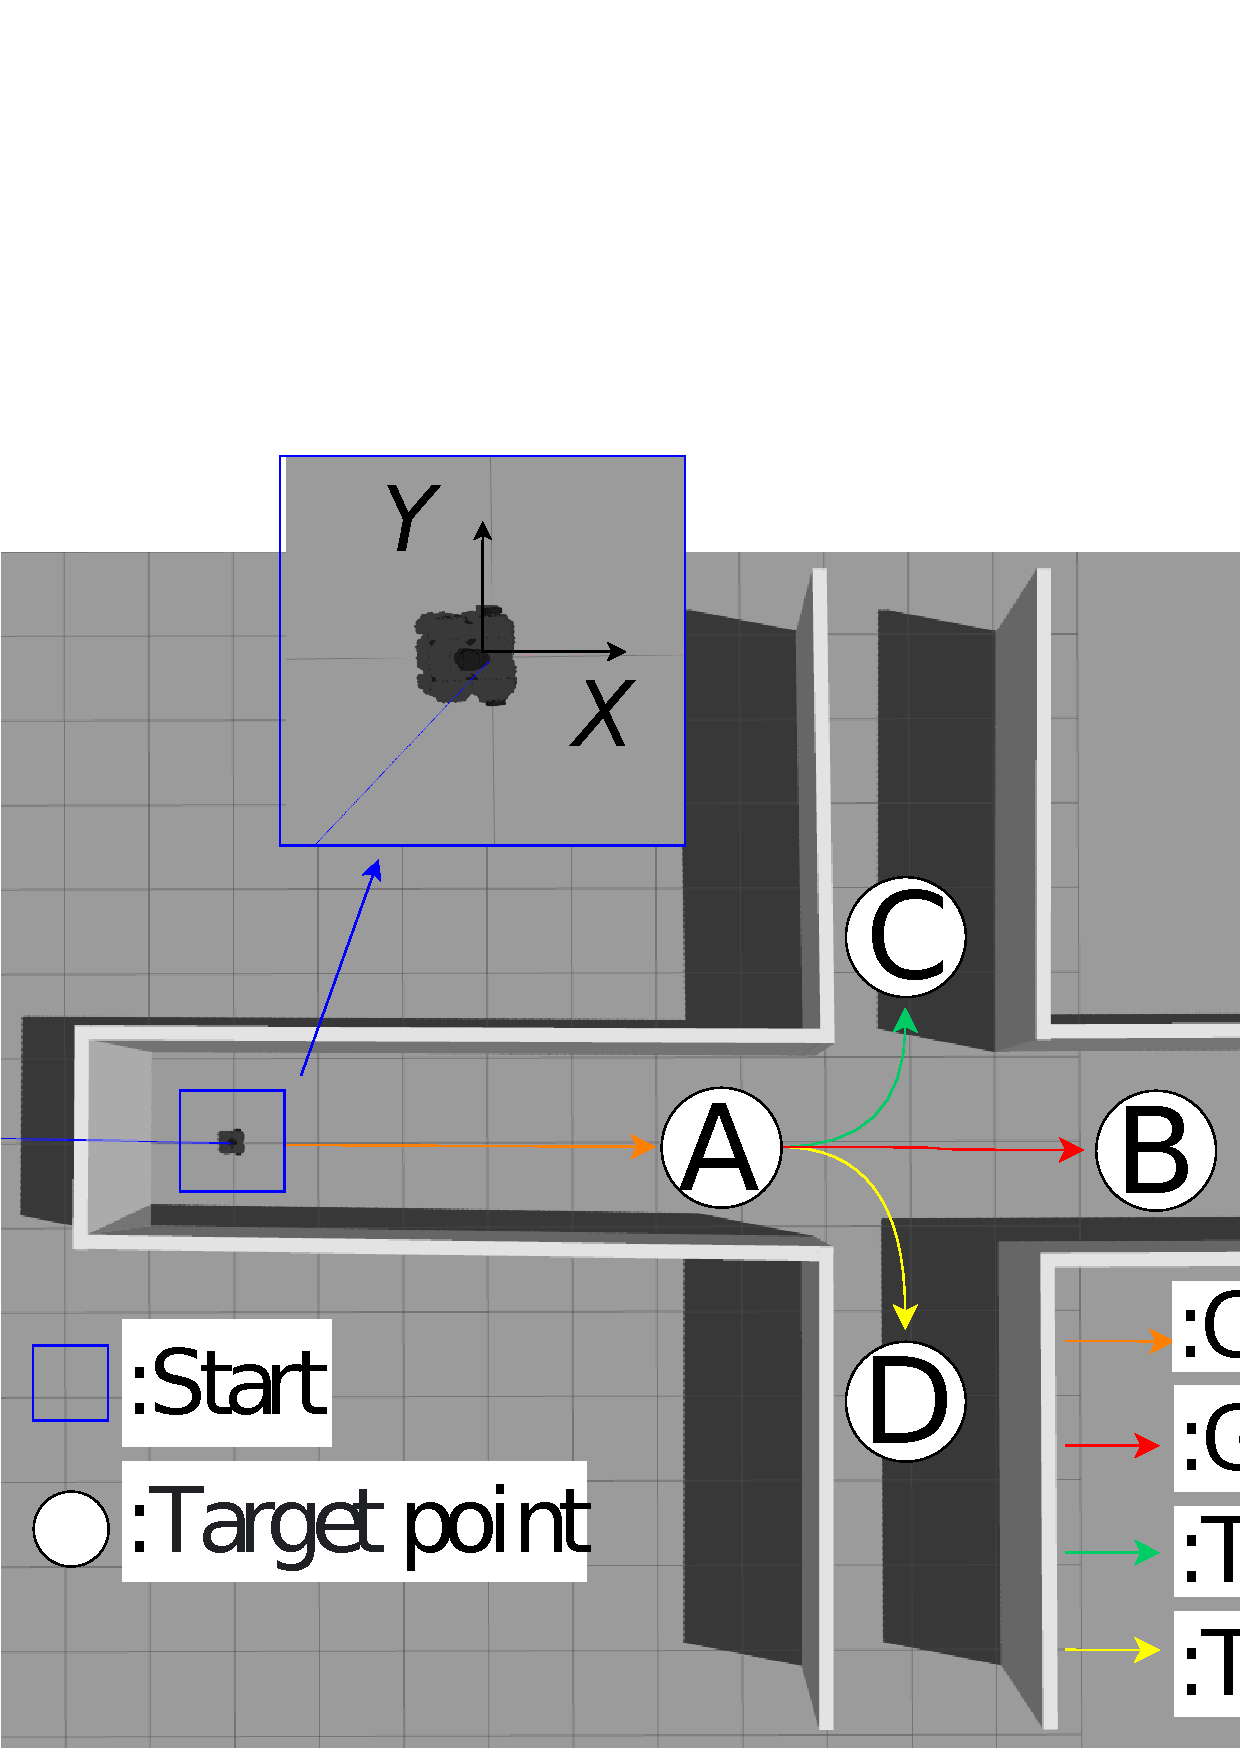
\includegraphics[width = 6.7cm]{./fig/zyuziroute.pdf}
            
            \caption{Environment and route for experiment}
            \vskip 0.1zh
            \label{fig:exp}
        \end{figure}
    \end{center}
    % \begin{enumerate}
    %     \setlength{\parskip}{0cm} % 段落間
    %     \setlength{\itemsep}{0cm} % 項目間
    %     \item 学習フェーズによって,学習器の訓練 ( 経路の学習 ) 行う
    %     ( 制御:地図べースの制御器の出力 )
    %     \item 設定した step 数を学習後,訓練フェーズへ移行
    %     ( 制御:学習器の出力 )
    %     \item コース内に設定した地点において目標方向のコマンドを入力,挙動を確認
    % \end{enumerate}
   \section{実験結果}
   実験結果を\reftab{suc}に示す.
   すべての経路において,目標地点へ到達することに成功した.
   結果から,目標方向指令によって経路を選択可能な
   機能を追加する提案手法の有効性が確認できた.
   \begin{table}[h]
    \caption{Number of successes experiment}
    \label{tab:suc}
    \begin{center}
        \vskip 0.5zh
        \begin{tabular}{|c|c|}
            \hline
            Route & Number of successes\\ \hline
            % Start - A (continue) & $10/10$ \\ \hline
            Start - A - B  & $10/10$ \\ \hline
            Start - A - C  & $10/10$ \\ \hline
            Start - A - D  & $10/10$ \\ \hline
        \end{tabular}
    \end{center}
\end{table}
    \section{結\hspace{2zw}言}%===========================
    本研究では,従来手法をベースに
    end-to-end学習による自律走行において,経路選択する機能の追加を提案した.
    またシミュレータを用いた実験により,機能の有効性を検証した.

    \vspace{5truemm}
    {\footnotesize
   
        \begin{thebibliography}{99}
            
            \bibitem{nvidia}
            Mariusz Bojarski et al:``End to End Learning for Self-Driving Cars'',
            arXiv: 1604.07316,(2016)
            \bibitem{okada}
            岡田眞也, 清岡優祐, 上田隆一, 林原靖男:``視覚と行動の end-to-end 
            学習により経路追従行動をオンラインで模倣する手法の提案''
        \end{thebibliography}
    }
    
    \normalsize
    
\end{document}
